\documentclass[conf]{new-aiaa}

\usepackage{float}
\usepackage{subfigure}
\usepackage[justification=centering]{caption}
\usepackage{multirow} \usepackage{graphicx}
\graphicspath{ {./images/} }
\usepackage{nameref}
\usepackage{amsmath}
\usepackage{amssymb}
\usepackage{amsfonts}
\usepackage[linesnumbered,ruled]{algorithm2e}
\usepackage{tikz}
\usetikzlibrary{calc,patterns,decorations.pathmorphing,decorations.markings,positioning,automata,shapes,arrows}
\tikzstyle{block} = [rectangle, draw, text width=3.5cm]
\tikzstyle{line} = [draw, -latex']
\usepackage{pgfplots}
\usepgfplotslibrary{colormaps,external}
\usepackage{ulem}
\usepackage{verbatim}
\usepackage[version=4]{mhchem}
\usepackage{siunitx}
\usepackage{pbox}
\usepackage{longtable,tabularx}
\setlength\LTleft{0pt} 

\title{Automated Wing Internal Structure Placement Guided by Finite Element Analysis}

\author{Justin L. Clough%
        \footnote{
          PhD Student, 
          Aerospace and Mechanical Engineering Department, 
          854 Downey Way, RRB 101.}
        and Assad A. Oberai%
        \footnote{  
          Professor, 
          Aerospace and Mechanical Engineering Department, 
          854 Downey Way, RRB 101.}}
\affil{University of Southern California,
       Los Angeles, CA, 90089}
\author{Andrew J. Zakrajsek%
        \footnote{
          Research Engineer,
          Air Force Research Laboratory, AFRL/RQ
          Bldg. 45, 2130 Eighth Street,
          Wright-Patterson AFB, OH 45433.}}
\affil{AFRL/RQHV, Wright-Patterson AFB,
       Dayton, OH, 45433}

\begin{document}
\maketitle

\begin{abstract}
The global structural design layout is typically missing 
in the early conceptual phase of aircraft design;
the internal structure itself is usually left uninitialized 
until the external geometry of the vehicle is finished.
This can lead to errors in the predicted performance 
of the aircraft.
This work details and demonstrates a program, \texttt{GRASP}, 
which automatically determines the optimal structural layout 
of traditional components (ribs and spars)
for use in this early design stage.
A user needed to only provide a wing outer mold line, 
material properties, vehicle weight, and allowable wing tip deflection.
A branch-and-cut style algorithm was implemented to explore the 
design space of possible rib and spar configurations.
For each configuration, a design flow of parametric geometry 
creation, discretization, and finite element analysis
was performed automatically using all open source software packages.
This was demonstrated for a wing and other parameters 
representative of the X-15 aeroplane.
The \texttt{GRASP} program calculated a optimal initial design layout
of 5 ribs and 2 spars in 139 minutes;
it evaluated a total of 11 different configurations
and successively selected the one which lowered 
wing tip deflection.
Future work includes adding a more representative 
loading conditions to match those seen in flight
and methods to decrease program run time.
\end{abstract}

\section{Nomenclature}

{\renewcommand\arraystretch{1.0}
\noindent\begin{longtable*}{@{}l @{\quad=\quad} l@{}}
GRASP & Guided Rib And Spar Placement \\
MER   & Mass Estimating Relations \\
FE    & Finite Element \\
AM    & Additive Manufacturing \\
OML   & Outer Mold Line \\
ESP   & Engineering Sketch Pad
\end{longtable*}}

\section{Introduction}
The conceptual design of modern aerospace systems is grounded in 
various multi-disciplinary design processes. 
These conceptual designs typically focus on the aerodynamic performance, 
weight assumptions, trajectory analysis, and overall ability of the 
system to meet the design requirements. 
A key discipline missing from the majority of early conceptual design, 
is the global structural design. 
This is due to the complex nature and knowledge required to 
design the internal structural layout of a new aerospace system 
\cite{horvath_aircraft_conceptual_structural_design_using_AMMIT,
      alyanak_efficient_supersonic_air_cehicle_structural_modeling,
      sensmeier_automatic_aircraft_structural_topology_generation_for_multidisc}.
Compounding this complexity is the ever changing vehicle 
geometry during the conceptual design phase, 
mainly due to recent advances in parametric geometry. 
Due to the early design fluidity, 
the conceptual structural design has been mainly incorporated in design 
loops through material selection and the resulting empirical 
Mass Estimating Relations (MERs) 
\cite{horvath_aircraft_conceptual_structural_design_using_AMMIT}.
These relations are used until the conceptual design is nearly finalized, 
which then initializes the structural design. 
The structural design typically starts with rough hand calculations, 
up to Finite Element (FE) methods, and eventual structural testing. 
At this point in the design cycle it is typically too late to greatly 
affect the overall system design 
\cite{alyanak_efficient_supersonic_air_cehicle_structural_modeling}.
Therefore, the final conceptual design can complicate the structural 
design and result in increased weight or reduced efficiency of the system. 
The early incorporation of structural design is important for understanding 
the proposed system’s feasibility, generating accurate weight predictions, 
assisting the multi-disciplinary design trade space exploration, 
and guiding the system to an optimal solution.

To generate rapid conceptual design trades, the structural layout 
and design should mainly be automated at the conceptual level. 
Automated structural design and layout has mainly been researched in 
two separate thrusts: 
(1) topology optimization, and  
(2) automated conventional structural optimization and layout. 
Advanced topology methods have been shown to produce optimal internal 
geometries with respect to minimizing stress, weight, and 
other key variables 
\cite{saitao_survey_of_structural_opt_2005,
      brampton_level_set_topology_optimisation_of_aircraft_wing_consdiring}.
While this research does show future benefit for the aerospace 
industry, it is also directly coupled to the current state of 
Additive Manufacturing (AM). 
A few of the top research challenges for AM when focused on aerospace 
system structures are:
understanding and predicting damage, machine to machine variability, 
print scale limitations, and cost of AM
\cite{ frazier_metal_additive_manufacturing_a_review,
       uriondo_the_present_and_future_of_AM_in_aerospace,
       wong_a_review_of_additive_manufacturing}.
Until these areas of research are better understood, 
AM is not currently a viable solution for traditional aerospace structures. 
With this understanding, this work focused on the near-term, 
benefits of automating the structural layout process and 
incorporating the results early in the conceptual design. 
While the automated structural layout can be considered a form of 
topology optimization, it will only be denoted as 
automated layout throughout this work.

Automating the structural layout process requires a specific and 
detailed focus on the design geometry, in addition to the selection 
of a structural analysis method. 
Recent research is focusing on incorporating structural design earlier 
in the design loop through automated hand calculation methods 
\cite{horvath_aircraft_conceptual_structural_design_using_AMMIT}.
This is aimed at incorporating initial structural design early in the design loop 
without the need for structural expertise. 
Adding to this other research has suggested that due to increased 
computational power, the inclusion of FE method
is possible early in conceptual design loop 
\cite{mason_conceptual_design_shop_tool_for_rapid_airframe_structural_modeling}.
There are benefits from incorporating the more detailed FE 
analysis early in the design loop, however, this also 
introduces new challenges, like automatic mesh generation. 
This issue is mainly addressed within the design framework.  
A structural optimization method was completed using FE analysis, 
automatic mesh generation, and a framework (python) environment 
\cite{hwang_geometry_and_structural_modeling_for_high_fidelity_aircraft_design_opt}.
The framework becomes extremely important for the incorporation of the structural 
design in the multi-disciplinary conceptual design loop. 
As the design and geometry change the structural design needs to adapt and change. 
This can be completed using parametric geometry, 
so the FE method and structural layout update as the vehicle design updates 
\cite{padula_structural_analysis_in_a_conceptual_design_framework}.
Using geometry as the center of an automated parametric design loop showed to be 
an important step for linking the structural design within the conceptual 
design loop 
\cite{lazzara_on_structural_layout_using_multifidelity_geometry_in_aircraft_design,
      bryson_framework_for_multifidelity_aeroelastic_vehicle_design_opt}.
Therefore, to truly bring automated structural design and placement 
early in the design loop, there needs to be a focus on common design 
geometry across disciplines and a framework capable of FE analysis. 
This leads to the ability to take a conceptual 
Outer Mold Line (OML) to an initial structural layout without the 
structural designer in the loop.

Completing the automatic structural layout at a conceptual level 
requires design knowledge held by structural experts. 
The vast majority of research in this area has looked at automatically 
laying out the structure by manually specifying the number of supports 
throughout the structure. 
This method still requires an engineer in the loop during the conceptual design. 
The manual layout of the initial structure for the conceptual design takes time, 
however, needs to be completed to allow a starting point for the FE analysis. 
For this work an initial structural placement will be completed using 
a branch-and-cut style algorithm
\cite{padberg_branch_and_cut_algorithm_for_resolution_of_sym_traveling_salesman}.
This will work to initialize the structural design and allow varying 
internal automated layouts to take place. 
The selection of the final automated layout can be performed following 
design constraints and objectives similar to topology 
optimization (minimize stress, etc.). 
Therefore, an OML can be entered into the loop, 
and the structural design model can continue to add supports while 
analyzing the structure to finalize an initial solution. 
Eventually, the goal would be to add an element of knowledge-based 
conceptual and preliminary structural design practices to this 
placement model 
\cite{anemaat_AAARaven_knowledge_based_aircraft_conceptual_and_prelim_design,
      niu_airframe_structural_design_practical_design_info_and_data_on_aircraft,
      sensmier_study_of_vehicle_structural_layouts_post_WWII_aircraft}.
While this is outside the work presented here, 
this area can become extremely beneficial for future conceptual 
structural designs as an ability to acquire a faster and higher 
fidelity automated conceptual structural design. 

The work presented here has the goal of highlighting the most 
advantageous method to achieve early automated structural conceptual 
designs, within the multi-disciplinary design loop 
independent of direct structural designer expertise. 
To accomplish this the automated layout process needs an OML input, 
design loads, and objective (i.e., minimize wing deflection below an allowable amount). 
The automation framework then should be linked to the same parametric geometry 
engine, a layout generation method, FE analysis, and a tailorable framework. 
The resulting work highlights how an 
automated conceptual design framework was setup to automate a 
structure layout without any input from the structural designer. 


\section{Methods} \label{sec:methods}
The goal was to develop an automated workflow to solve an 
optimal parametric structural layout problem. 
In this problem, a user specifies a design constraint that must be satisfied, 
and a set of integer parameters that define the geometry of the structure. 
The goal is to find an optimal value of these parameters that would achieve 
the design constraint. 
In the specific problem considered, the 
design constraint is a bound on the maximum allowable tip deflection of 
a wing under a prescribed loading, the integer parameters are the number 
of ribs and spars in the wing, and the goal is to find the smallest 
number of spars and ribs that would achieve the tip-deflection constraint. 

In order to solve this problem, the workflow 
described in Figure \ref{fig:design_flow} was developed.
Here the first portion is a geometry creation component, 
which given the value of the parameters of interest, 
generates the geometry of the structure. 
The second component further processes this geometry and generates 
a FE mesh for it. 
The third component uses this mesh to solve a structural analysis 
problem and evaluates the value of the design constraint. 
Once this workflow is established, it may be used to solve the optimal 
structural design problem using an appropriate integer programming algorithm. 
Since the focus of this paper is to demonstrate how this workflow 
can be established, a simple integer optimization 
algorithm, that is the branch-and-cut method, was used to solve this problem
\cite{padberg_branch_and_cut_algorithm_for_resolution_of_sym_traveling_salesman}. 
This algorithm proceeds as follows:

\begin{enumerate}
  \item Start with an initial configuration that does not satisfy the design constraint. 
  \item Increment each integer parameter by 1, 
          and use the workflow to generate multiple designs and to determine 
          the design constraint for each design.
  \item If the design constraint is satisfied by one or more designs, the problem is solved. 
  \item If no design satisfies the constraint, select the one that provided the largest 
          drop in the constraint, and go to Step 2. 
\end{enumerate}

\noindent
The different configurations formed the nodes of a tree which was 
traversed in a depth-first manner.
An example of this tree is shown in Figure \ref{fig:decision_tree}.

\begin{figure}[H]
  \centering
  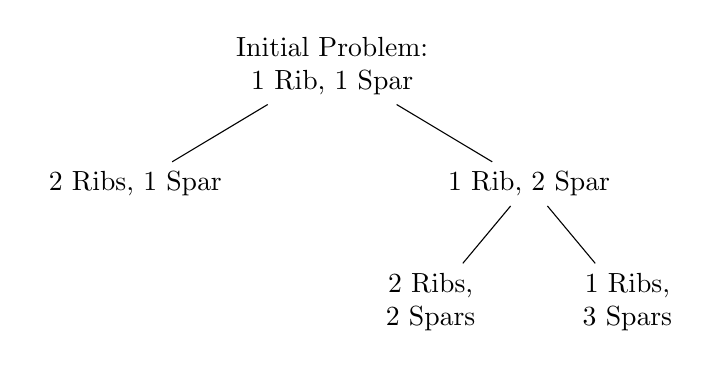
\begin{tikzpicture}[
      level distance=1.5cm,
      level 1/.style={sibling distance=5cm},
      level 2/.style={sibling distance=2.5cm}]
    \node[text width=2.5cm, align=center] {Initial Problem:  1 Rib, 1 Spar}
        child 
          { node [text width=2.5cm, align=center]{2 Ribs, 1 Spar} }
        child 
          {
          node[text width=2.5cm, align=center] {1 Rib, 2 Spar} 
            child {node [text width=1.5cm, align=center]{2 Ribs, 2 Spars}}
            child {node[text width=1.5cm, align=center] {1 Ribs, 3 Spars}}
          };
  \end{tikzpicture}
  \caption{Example decision tree with configurations as nodes.}
  \label{fig:decision_tree}
\end{figure}

A python script, \texttt{GRASP}\footnote{\texttt{GRASP} repository at \texttt{github.com/JustinClough/grasp}}, 
(Guided Rib And Spar Placement)
was written to implement the design flow logic
and to operate the branch-and-cut algorithm.
This design flow is shown in Figure \ref{fig:design_flow};
it includes 
component creation,
geometry management and discretization,
and the FE analysis.

\begin{figure}[H]
  \centering
  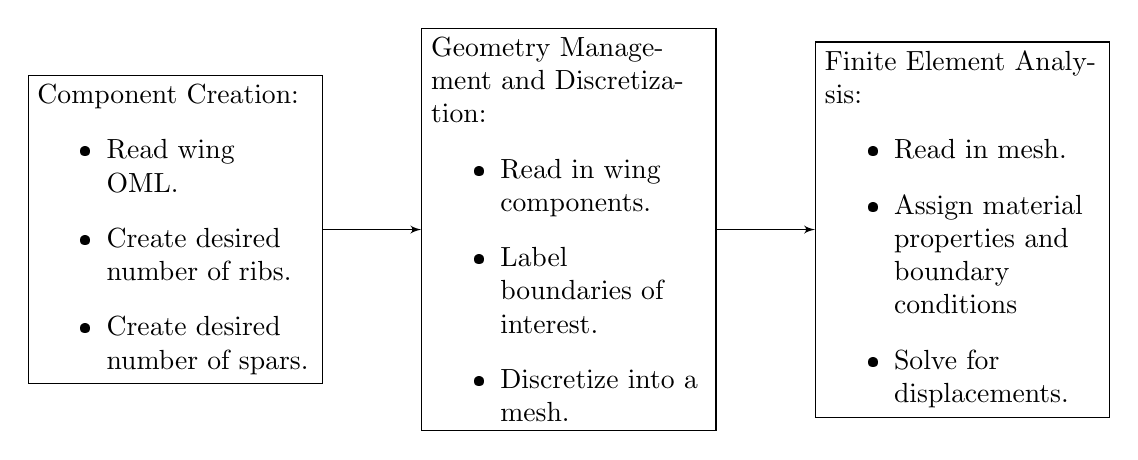
\begin{tikzpicture}[node distance = 5cm, auto]
    % Blocks
    \node [block] (geom) 
    {
      Component Creation:
      \begin{itemize}
        \item Read wing OML.
        \item Create desired number of ribs.
        \item Create desired number of spars.
      \end{itemize}
    };
    \node [block, right of=geom] (mesh) 
    {
      Geometry Management and Discretization:
      \begin{itemize}
        \item Read in wing components.
        \item Label boundaries of interest.
        \item Discretize into a mesh.
      \end{itemize}
    };
    \node [block, right of=mesh] (fea)  
    {
      Finite Element Analysis:
      \begin{itemize}
        \item Read in mesh.
        \item Assign material properties and boundary conditions
        \item Solve for displacements.
      \end{itemize}
    };
    % Lines
    \path [line] (geom) -- (mesh);
    \path [line] (mesh) -- (fea);
  \end{tikzpicture}
  \caption{Automatic design flow logic and steps.}
  \label{fig:design_flow}
\end{figure}

\noindent
Templated base input files were created for use with each 
of the subprograms used at each step of the design flow.
The python script edited the corresponding input file for the specific problem 
configuration.
It then called each subprogram in the necessary order.

The script based geometry kernel
\texttt{Engineering Sketch Pad} (\texttt{ESP})
was used to create a geometry of a problem of interest
\cite{haimes_ESP_solid_modeling_feature_based_web_enabled_system_param_geom}.
For this study, the base geometry was the right wing
of the X-15, borrowed from 
\cite{gochenaur_rapid_geometry_generation_and_basic_comparison_x15}.
This geometry was then populated with ribs and spars;
these components each had a prescribed thickness.
The ribs and spars
were written to disk and then read into \texttt{Gmsh} 
\cite{geuzaine_GMSH_3D_FE_mesh_generator}.
This software then joined all components together through
boolean fragmentation and unions to form a single solid geometry. 
It then was used to produce a second order 
tetrahedral mesh discretization of this geometry.
The FE analysis software \texttt{Albany} 
\cite{salinger_albany_using_component_based_design_to_dev_flex_multiphysics}
then read in this mesh, 
solved a linear elastic problem, 
and calculated the deformation and stresses of the geometry 
in the wing under a predefined load condition.
Each of these design flow steps are described in detail 
in the following subsections.

\subsection{Parametric Geometry with \texttt{ESP}} \label{sec:meth_esp}
Two sets of two \texttt{.udc} files were written to allow a user to 
parametrically place ribs and spars for any wing shape. 
A \texttt{.udc} file contains a user defined function.
One of these files, \texttt{make\_rib.udc}, allows the user 
to place a rib at a specified percent-span.
The other in this set is \texttt{even\_ribs.udc};
this calls \texttt{make\_rib.udc} to place a user defined number of ribs
evenly throughout the span of the wing.
A similar set of programs were created for spar placement.

A templated input script was created and used for 
each problem configuration considered.
The numbers of ribs and spars were automatically edited.
Next, the \texttt{ESP} binary was called as a subprocess.
The geometries created by these scripts were then written to 
disk as \texttt{.stp} files
\cite{iso_10303_21_2016_step_files}.
Each component was written in its own \texttt{.stp} file.
The generic method was \texttt{rib\_R.stp} contained all
geometric information of rib number $R$;
\texttt{spar\_S.stp} contained all
geometric information of spar number $S$.
When finished, the output was checked for errors.

Three main types of wing shapes were tested to verify the \texttt{.udc} 
files worked as expected.
The three wing shapes were Standard, Double Delta, and Double Dihedral. 
Examples of these shapes are shown in Figure \ref{fig:no_internals}.

\begin{figure}[H]
  \centering
  \subfigure[Standard.]
    {
      \includegraphics[width=0.25\textwidth, height=0.25\textwidth]
      {x15_iso}
    }
  \subfigure[Double Delta.]
    {
      \includegraphics[width=0.25\textwidth, height=0.25\textwidth]
      {double_delta_iso}
    }
  \subfigure[Double Dihedral.]
    {
      \includegraphics[width=0.25\textwidth, height=0.25\textwidth]
      {double_di_iso}
    }
  \caption{
      Geometries of the three base wing types.}
  \label{fig:no_internals}
\end{figure}

\noindent
The rib and spar file sets were then able to be read into \texttt{Gmsh}.
The tessellation automatically performed by \texttt{ESP} was not used 
for the FE analysis.

\subsection{Geometry Management and Discretization} \label{sec:meth_geom}
A template \texttt{Gmsh} script file was created and automatically 
edited for each problem configuration.
The script first read the first spar and rib from disk.
It then used boolean fragmentation and unions to form a new 
single continuous volume from the two components. 
The next component was then read from disk and added to the union
in a similar method. 
This was repeated for all components until a single volume was formed
that had all ribs and spars.

Boundaries of interest were then automatically found and labeled. 
This included the wing root surfaces and the wing underside.
Each spar root surface was found by identifying the surface enclosed in 
a thin bounding box near the wing root and at the corresponding percent chord.
The wing underside was determined as the surface with the 
lowest boundary.
These surfaces were labeled such that boundary conditions 
could be applied during the FE analysis step.

The geometry was then discretized into second order tetrahedral elements. 
A size field was specified such that at least two elements
spanned any geometric feature.

\subsection{Finite Element Model} \label{sec:meth_FEM}
Two template \texttt{Albany} input files were created 
and automatically edited for each problem configuration.
The first file dictated boundary conditions and linear algebra solver parameters.
The second file specified material information such as model type and properties.

A linear elastic material model was used.
The user specified the Young's modulus and Poisson ratio for the material. 
All components of the wing used the same material model and properties.
The elements used were 10-node composite tetrahedrons
\cite{ostien_10_node_comp_tet_FE_for_solid_mechanics}.
These elements were chosen after testing in order to
ensure that they did not suffer from shear locking
often observed in some standard FE formulations.

All degrees of freedom on the wing root surface were assigned
a homogeneous Dirichlet boundary condition.
The underside of the wing was assigned a
Neumann boundary condition of a uniform upward traction.
The magnitude of this traction was calculated by distributing
a user defined total weight over the lower surface area.
This was to represent the lift from airflow over the wing.

\subsection{Workflow Demonstration} \label{sec:meth_demonstration}
Wing tip deflection was brought below a prescribed allowable level
using the \texttt{GRASP} program for a example aircraft.
The OML of the X-15 was used as the base wing geometry 
\cite{gochenaur_rapid_geometry_generation_and_basic_comparison_x15}.
Material properties of Ti6Al4V were used;
these were a Young's modulus of 113.8 GPa and
a Poisson's ratio of 0.342 \cite{boyes_materials_properties_handbook_titanium_alloys}.
A weight of 123.0 KN, representing the full weight of the X-15 
\cite{gochenaur_rapid_geometry_generation_and_basic_comparison_x15},
was distributed uniformly as an upward pressure over the bottom face of the wing.
This approximated the load of a 2G maneuver on the wing frame.
The spars were created with thicknesses of 30 mm;
ribs had a thickness of 5 mm.
An allowable tip deflection of  5 cm was used.

\section{Results} \label{sec:results}
Images showing the internal geometries created by the \texttt{.udc} 
files are shown for verification of expected function behavior.
This includes internal views for both the Double Delta 
and Double Dihedral wings.
Images and plots from the tip deflection demonstration are 
presented as well.
These include a surface plot tip deflection 
with respect to considered configurations
and images of meshes used for the FE model.
Solution times and timing breakdowns are also shown.


\subsection{Validation of \texttt{.udc} Files} \label{sec:validation}
The \texttt{.udc} files were tested on the Double Delta and Double Dihedral 
wing types shown in Figure \ref{fig:no_internals}. 
Figure \ref{fig:fewSomeMany} shows the variability of the number
of internal components which can be placed.
An isometric view of the internal components for the Double Delta 
wing is shown in Figure \ref{fig:delt_in_out};
a similar view for the Double Dihedral is shown in Figure \ref{fig:di_in_out}.
Images show components with zero thickness for clarity.

\begin{figure}[H]
  \centering
  \subfigure[Few internal components.]
    {
      \includegraphics[width=0.30\textwidth, height=0.30\textwidth]
      {double_delta_few}
    }
  \subfigure[Mixed number of internal components.]
    {
      \includegraphics[width=0.30\textwidth, height=0.30\textwidth]
      {double_delta_mixed}
    }
  \subfigure[Many internal components.]
    {
      \includegraphics[width=0.30\textwidth, height=0.30\textwidth]
      {double_delta_many}
    }
  \caption{
        Double delta wing with differing numbers of parametrically placed 
        internal supports. }
  \label{fig:fewSomeMany}
\end{figure}

\begin{figure}[H]
  \centering
  \subfigure[External view.]
    {
      \includegraphics[width=0.45\textwidth, height=0.25\textwidth]
      {double_delta_iso_out}
    }
  \subfigure[Top surface removed.]
    {
      \includegraphics[width=0.45\textwidth, height=0.25\textwidth]
      {double_delta_iso_in}
    }
  \caption{
        Double delta wing with and without top surface to show
        geometries of the internal components.}
  \label{fig:delt_in_out}
\end{figure}

\begin{figure}[H]
  \centering
  \subfigure[External view.]
    {
      \includegraphics[width=0.45\textwidth, height=0.25\textwidth]
      {double_di_ext}
    }
  \subfigure[Top surface removed.]
    {
      \includegraphics[width=0.45\textwidth, height=0.25\textwidth]
      {double_di_in}
    }
  \caption{
        Double dihedral wing with and without top surface to show
        geometries of the internal components.}
  \label{fig:di_in_out}
\end{figure}

\subsection{Demonstration Of Full Workflow}
A surface plot generated by computing the 
tip deflection for numbers of ribs and spars is shown in 
Figure \ref{fig:tip_deflection_surface}.
A spar and rib thickness of 30 mm and 4 mm, respectively, was used
along with the geometry and weight for the X-15.
This shows the sensitivity of the deflection at the
tip of the wing to various configurations of 
ribs and spars.

\begin{figure}[H]
  \centering
  \begin{tikzpicture}
    \begin{axis} [
        xlabel={Spars}, 
        ylabel={Ribs}, 
        zlabel={Tip Deflection (m)},
        zmax=5.0,
        grid=both,
        grid style={line width=.1pt, draw=gray!10},
        major grid style={line width=.2pt,draw=gray!50},
        xtick={},
        ytick={},
        zmode=log,
        colormap/bluered,
        view={135}{45}]
      \addplot3 [patch, patch table={data/triangles.txt}] 
        table {data/surface_plot_data.txt};
    \end{axis}
  \end{tikzpicture}
  \caption{ 
    Tip deflection with respect to numbers of ribs and spars. }
  \label{fig:tip_deflection_surface}
\end{figure}

The maximum tip deflection was for the 
1-rib, 1-spar configuration and was 14.6 meters.
The minimum tip deflection was 5.9 mm for
the 8-rib, 8-spar configuration.

A demonstrative problem was run to test the entire workflow. 
In this problem the goal was to find the integer combination of 
ribs and spars that produced a tip deflection for a X-15 wing 
less than 5 cm with the fewest number of total components. 
The initial configuration was a wing with a single rib and spar. 
The skin of the wing was not modeled;
it was determined that it 
did not provide significant bending stiffness to the structure. 
The entire load on the wing, equal to 123.0  KN, was 
distributed uniformly on the lower surface of the ribs and spars.

The path selected by the optimization algorithm is shown 
in Table \ref{tab:solution_path} and Figure \ref{fig:x15_solution_path}.
The algorithm reached the prescribed constraint in 5 steps.
Each step required the generation of two configurations 
and the solutions of the corresponding structural problems.
The final configuration comprised of 5 ribs and 2 spars produced 
a tip deflection of 3.62 cm. 
As shown in Figure \ref{fig:x15_solution_path}, 
the algorithm added the second spar in the second step 
and thereafter always preferred adding a rib over another spar.

\begin{table}[H]
  \centering
  \caption{
      Intermediate configurations and deflections.  }
  \begin{tabular}{| c | c | c | c |}
    \hline
    Step Number & Ribs  & Spars & Displacement [mm] \\ 
    \hline
    0 & 1 &  1        &  4040.0             \\
    1 & 2 &  1        &   966.7             \\
    2 & 2 &  2        &   345.5             \\
    3 & 3 &  2        &   137.0             \\
    4 & 4 &  2        &    66.3             \\
    5 & 5 &  2        &    36.2             \\
    \hline
  \end{tabular}
  \label{tab:solution_path}
\end{table}


\begin{figure}[H]
  \centering
  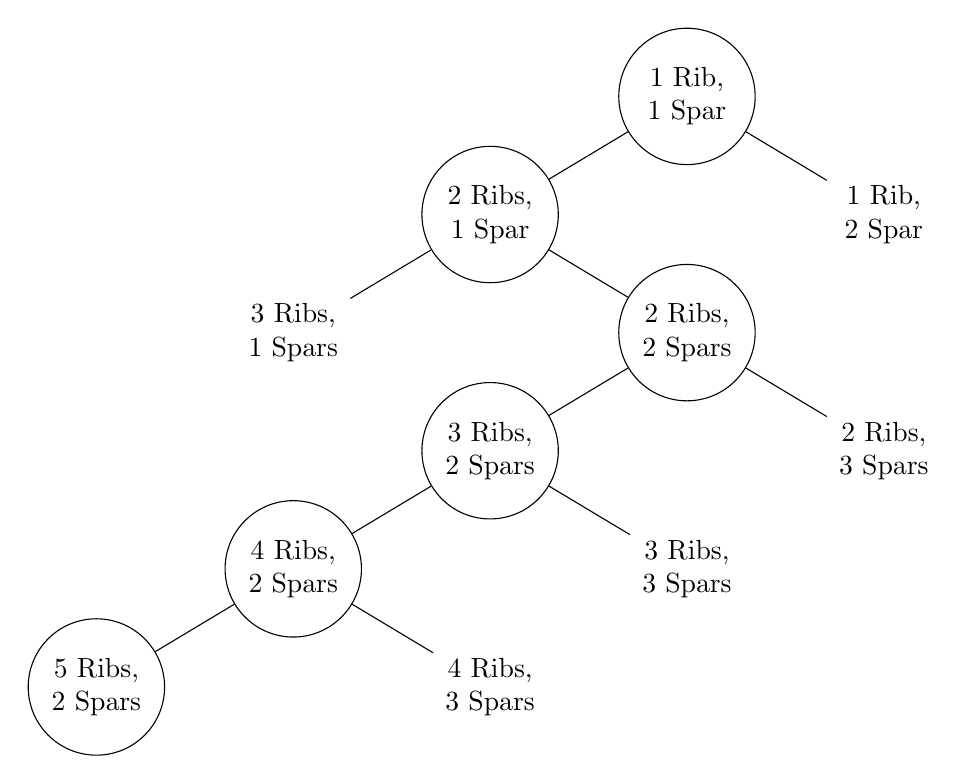
\begin{tikzpicture}[
      level distance=1.5cm,
      level 1/.style={sibling distance=5cm},
      level 2/.style={sibling distance=2.5cm}
      level 3/.style={sibling distance=2.5cm}
      level 4/.style={sibling distance=2.5cm}
      level 5/.style={sibling distance=2.5cm}]
    \node[circle,draw, text width=1.2cm, align=center] {1 Rib, 1 Spar}
        child 
          { node [circle,draw, text width=1.2cm, align=center]{2 Ribs, 1 Spar} 
            child 
            { node [text width=1.2cm, align=center]{3 Ribs, 1 Spars}}
            child 
            { node[circle,draw, text width=1.2cm, align=center] {2 Ribs, 2 Spars}
              child 
              { node[circle,draw, text width=1.2cm, align=center] {3 Ribs, 2 Spars}
                child 
                { node[circle,draw, text width=1.2cm, align=center] {4 Ribs, 2 Spars}
                  child 
                  { node[circle,draw, text width=1.2cm, align=center] {5 Ribs, 2 Spars}
                  }
                  child 
                  { node[text width=1.2cm, align=center] {4 Ribs, 3 Spars}
                  }
                }
                child 
                { node[text width=1.2cm, align=center] {3 Ribs, 3 Spars}
                }
              }
              child 
              { node[text width=1.2cm, align=center] {2 Ribs, 3 Spars}
              }
            }
          }
        child 
          { node[text width=1.2cm, align=center] {1 Rib, 2 Spar} };
  \end{tikzpicture}
  \caption{Path taken by \texttt{GRASP} to build wing frame.
           Configuration that lowered tip deflection is circled 
            at each level.}
  \label{fig:x15_solution_path}
\end{figure}

The value of tip deflection at each step for the two configurations 
that were evaluated, one with an extra rib and another with an extra spar,
is shown in Figure \ref{fig:tip_deflection_steps}.
It was observed that except for the second step, 
the tip deflection produced by adding an extra rib was 
smaller than that produced by adding and extra spar. 


\begin{figure}[H]
  \centering
    \begin{tikzpicture}
      \begin{axis}[
        legend pos=outer north east,
        legend cell align={left},
        grid=both,
        grid style={line width=.1pt, draw=gray!10},
        major grid style={line width=.2pt,draw=gray!50},
        xtick={},
        ytick={},
        ymode=log,
        minor tick num=5,
        xlabel=Step Number,
        title=Tip Deflection At Each Step,
        ylabel={Tip Deflection [mm]} ]
        \addplot table {data/deflection_steps_ribs.txt};
          \addlegendentry{Added Rib}
        \addplot table {data/deflection_steps_spars.txt};
          \addlegendentry{Added Spar}
      \end{axis}
    \end{tikzpicture}
  \caption{ Tip deflection with respect to the number of steps taken
            for adding either a rib or spar.}
  \label{fig:tip_deflection_steps}
\end{figure}

The total computer time required for generating 
and solving the two configurations at each step is shown 
in Figure \ref{fig:solution_time_steps}.
The solution time grows by a factor of 10 between 
the first and the last step. 
This is because with each step as more components are added to the model, 
the effort required to construct and mesh the geometry 
and then to solve the corresponding FE problem increases. 
At each step the time required to solve the problem with an extra rib 
was 21\% to 32\% more than the time required for the extra spar problem. 
This can be attributed to the extra effort required in 
meshing the thin region near the trailing edge.
This plot also illustrates the advantage of
using the branch-and-cut algorithm over an exhaustive search;
spanning the entire parameter space would become prohibitive
with the increasing number of components in the latter approach.

\begin{figure}[H]
  \centering
    \begin{tikzpicture}
      \begin{axis}[
        legend pos=outer north east,
        legend cell align={left},
        grid=both,
        grid style={line width=.1pt, draw=gray!10},
        major grid style={line width=.2pt,draw=gray!50},
        xtick={},
        ytick={},
        minor tick num=5,
        xlabel=Step Number,
        title=Solution Time At Each Step,
        ylabel={Time [s]} ]
        \addplot table {data/total_time_steps_ribs.txt};
          \addlegendentry{Added Rib}
        \addplot table {data/total_time_steps_spars.txt};
          \addlegendentry{Added Spar}
      \end{axis}
    \end{tikzpicture}
  \caption{ Time to calculate solution for each configuration 
            with respect to the number of steps taken
            for adding either a rib or spar.}
  \label{fig:solution_time_steps}
\end{figure}

The number of finite elements generated for the two configurations 
at each step of the algorithm are 
shown in Figure \ref{fig:num_elements_steps}.
These increase by 5,000 to 10,000 with each step 
and rise to a total of 50,0330 for the final evaluated configuration.
On average, spars and ribs required roughly 
9000 and 5000 elements to model, respectively.

\begin{figure}[H]
  \centering
    \begin{tikzpicture}
      \begin{axis}[
        legend pos=outer north east,
        legend cell align={left},
        grid=both,
        grid style={line width=.1pt, draw=gray!10},
        major grid style={line width=.2pt,draw=gray!50},
        xtick={},
        ytick={},
        minor tick num=5,
        xlabel=Step Number,
        title=Number Of Elements At Each Step,
        ylabel={Number of Elements} ]
        \addplot table {data/elements_steps_ribs.txt};
          \addlegendentry{Added Rib}
        \addplot table {data/elements_steps_spars.txt};
          \addlegendentry{Added Spar}
      \end{axis}
    \end{tikzpicture}
  \caption{ Finite elements in each mesh for each configuration
            compared to the number of steps taken
            for adding either a rib or spar.}
  \label{fig:num_elements_steps}
\end{figure}

Table \ref{tab:solution_time_breakdown} provides a break-down of the 
computational time spent in the three main components of the workflow: 
geometry creation in \texttt{ESP}, 
geometry processing and mesh generation in \texttt{Gmsh}, 
and FE analysis in \texttt{Albany}. 
For the initial configuration, the time spent in \texttt{Gmsh} 
and \texttt{Albany}
was similar and was three times the time spent in \texttt{ESP}. 
However, for the final few configurations the situation was reversed;
here most of the time was spent in combining the different components 
and then meshing them in \texttt{Gmsh}. 
Remarkably the time required for the FE analysis 
was less than a tenth of this time.
This may be attributed to the advanced solvers and preconditioners 
used within 
\texttt{Albany} 
\cite{salinger_albany_using_component_based_design_to_dev_flex_multiphysics}.
The program took a total of 139 minutes to run on a Linux
workstation with a i5-7400 CPU which had a clock speed of 3 GHz.

\begin{table}[H]
  \centering
  \caption{
    Time in each portion of the design flow throughout 
    evaluated configurations. All times in seconds.}
  \begin{tabular}{| c | c | c | c | c | c |}
    \hline
    Step Number & Ribs  & Spars & Geometry Creation & Geometry Management and Discretization & FE Analysis\\
    \hline
    0 & 1 &  1        & 13 & 39 & 39    \\
    1 & 2 &  1        & 14 & 66 & 89    \\
    2 & 2 &  2        & 14 & 287 & 69   \\
    3 & 3 &  2        & 16 & 656 & 91   \\
    4 & 4 &  2        & 16 & 1206 & 112 \\
    5 & 5 &  2        & 16 & 1871 & 122 \\
    \hline
  \end{tabular}
  \label{tab:solution_time_breakdown}
\end{table}

In Figure \ref{fig:all_meshes}, 
the geometry and the mesh at each step are plotted;
in Figure \ref{fig:all_solutions}
the deformed shape of the configuration is shown.
In this figure, for each configuration, 
the surface is colored with the magnitude of displacement.
The maximum deflection occured at the tip of the spar closer to the leading edge, 
and that with each new rib that was added the magnitude of this displacement, 
as well as the difference between the tip deflection of this spar 
and the one downstream of it, reduced. 

\begin{figure}[H]
  \centering
  \subfigure[Step 0: 1 Rib, 1 Spar.]
    {
      \includegraphics[width=0.45\textwidth, height=0.30\textwidth]
      {mesh_1_1}
    }
  \subfigure[Step 1: 2 Rib, 1 Spar.]
    {
      \includegraphics[width=0.45\textwidth, height=0.30\textwidth]
      {mesh_2_1}
    }
  \subfigure[Step 2: 2 Rib, 2 Spar.]
    {
      \includegraphics[width=0.45\textwidth, height=0.30\textwidth]
      {mesh_2_2}
    }
  \subfigure[Step 3: 3 Rib, 2 Spar.]
    {
      \includegraphics[width=0.45\textwidth, height=0.30\textwidth]
      {mesh_3_2}
    }
  \subfigure[Step 4: 4 Rib, 2 Spar.]
    {
      \includegraphics[width=0.45\textwidth, height=0.30\textwidth]
      {mesh_4_2}
    }
  \subfigure[Step 5: 5 Rib, 2 Spar.]
    {
      \includegraphics[width=0.45\textwidth, height=0.30\textwidth]
      {mesh_5_2}
    }
  \caption{
      Meshes used at different solution steps.}
  \label{fig:all_meshes}
\end{figure}

\begin{figure}[H]
  \centering
  \subfigure[Step 0: Scale of 0.1.]
    {
      \includegraphics[width=0.45\textwidth, height=0.30\textwidth]
      {deformed_1_1}
    }
  \subfigure[Step 1: Scale of 1.0.]
    {
      \includegraphics[width=0.45\textwidth, height=0.30\textwidth]
      {deformed_2_1}
    }
  \subfigure[Step 2: Scale of 1.0.]
    {
      \includegraphics[width=0.45\textwidth, height=0.30\textwidth]
      {deformed_2_2}
    }
  \subfigure[Step 3: Scale of 5.0.]
    {
      \includegraphics[width=0.45\textwidth, height=0.30\textwidth]
      {deformed_3_2}
    }
  \subfigure[Step 4: Scale of 10.]
    {
      \includegraphics[width=0.45\textwidth, height=0.30\textwidth]
      {deformed_4_2}
    }
  \subfigure[Step 5: Scale of 20.]
    {
      \includegraphics[width=0.45\textwidth, height=0.30\textwidth]
      {deformed_5_2}
    }
  \caption{
        Mesh at each step with displacement magnitude contour plot and
        deformed with the displacement vector;
        scale factors used to show deflections.}
  \label{fig:all_solutions}
\end{figure}

\section{Discussion and Closing Remarks} \label{sec:closing_remarks}
The \texttt{GRASP} program was able to solve
an optimal parametric structural layout problem by
automatically creating an initial frame design.
A user specified design constraint, maximum allowable wing deflection, 
was satisfied by determining the integer numbers of ribs and spars
to populate the wing frame for a demonstrated vehicle.
A simplified version of the branch-and-cut method was used
to step through possible configurations.
For each configuration, a design flow consisting of
component creation, geometry discretization, and a FE analysis
was executed.

The components of the wing frame were created 
using the parametric, script-based, geometry kernel \texttt{ESP}.
Each component was written to disk and 
then read into \texttt{Gmsh} automatically.
The components were then unioned together to form one
continuous volume which represented the wing frame.
Boundaries of interest were tagged and the 
volume was discretized into a FE mesh which was written to disk.
This mesh was then read into \texttt{Albany}
where boundary conditions and material properties 
were assigned.
The FE problem was then solved for nodal displacements.

The demonstration shows that the \texttt{GRASP} program was able to 
create a design for the frame of a wing OML automatically
in approximately 2 hours. 
In this time it considered 11 different configurations
and successively chose the one which lowered tip deflection.
This was done using all open-source software packages.

This work demonstrates a viable method to bring structural layout 
into the initial design phase for aircraft.
It does so without the need for a structural design 
specialist present.
This will benefit the air vehicle design community 
by introducing greater modeling accuracy 
earlier in the design process. 
In turn this will lead to aircraft designs
which more efficiently meet their design criteria.
Additionally, layouts generated using \texttt{GRASP}
rely on traditional and tested manufacturing methods.


\section{Future Work} \label{sec:future}
Possible improvements would include allowing for different 
materials throughout the wing, modeling the wing skin with stringers, 
and testing under more load cases.
These additions would allow for more accurate modeling 
of the wing in use.

Allowing for different components to have different
material properties would generalize the given method.
Some but not all wing constructions use the same material
throughout the wing. 
For example, the X-15 used both Inconel and Titanium alloys
in its wing construction,
\cite{ kordes_structural_heating_experiences_on_the_x15,
       price_design_report_thermal_protection_system_x15A_2},
whereas a commercial Cessna uses the same Aluminum alloy
throughout the wing, only differing by temper 
\cite{cessna_maintenance_manual_single_engine_models_1996}.
Additionally, different material models could be used 
on different components.
These models would include the pertinent physical behavior
needed to understand the performance of the design.
Including the wing skin and stringers would also 
increase the general accuracy of the model.
This would be especially important for more complex
load cases where the stringers and skin must 
distribute the aerotractions to the ribs and spars.
Lastly, more complex load cases could be
created and designed for to better represent those in flight.

The \texttt{GRASP} software can also be
made faster by a few methods. 
First, configurations can be processed in parallel;
this would decrease the total solution time 
to near half.
Second, both \texttt{Gmsh} and \texttt{Albany}
are able to operate in parallel 
\cite{salinger_albany_using_component_based_design_to_dev_flex_multiphysics,
      geuzaine_GMSH_3D_FE_mesh_generator}.
Calling these application with parallel resources
would also decrease the time to solve each configuration.
Finally, each step of the design flow
shown in Figure \ref{fig:design_flow} starts and
end with reading a writing to the disk. 
Processing fully in memory without the 
file input/output would also 
decrease the total time to calculate solutions.


\section*{Acknowledgments}
The authors thank the DoD Science, Mathematics, And 
Research for Transformation (SMART) Scholarship
for Service Program which sponsored this work.


\bibliography{monolith.bib}

\end{document}
